This section introduces the preparation of our experiments to evaluate our proposed framework.
For this purpose, we have deployed an \textit{SDP} network, generated traffic simulating normal behavior to train an
\textit{IDS} model and trained our framework to generate adversarial traffic.

The code that was used and created during the evaluation of our proposal is completely open and accessible.
It can be found on the popular code sharing and collaboration platform,
\textit{GitHub}~\footnote{https://github.com/antonioalfa22/Harpe}.

\subsection{Methodology}\label{subsec:methodology}
To evaluate the performance of our proposed framework, we have designed two environments to test its ability to
generate adversarial traffic that can fool an ML-based \textit{IDS}.

To evaluate the performance of our solution, we first employed \textit{IDS} datasets from previous studies that were
used in traditional network architectures in our test environment.
This approach allows us to assess our solution's ability to generate adversarial traffic that can evade detection by
existing classifiers
Finally, we have developed a second environment to test our solution in an SDP-based network.
The objective of this evaluation environment is to assess the ability of our solution to generate adversarial traffic
that can evade detection by the \textit{IDS} in the \textit{SDP Controller}.
This will provide a comprehensive understanding of the effectiveness of our solution in modern network environments
and its potential to circumvent security mechanisms.

In this study, we have specifically focused on evaluating the performance of our solution against denial of service
\textit{(DoS)} attacks.
This is because \textit{DoS} attacks are a prevalent type of attack and are present in all of the datasets used in our
analysis.
Despite the presence of other types of attacks in these datasets, focusing on \textit{DoS} attacks allows us to have a
specific and consistent benchmark to evaluate our solution's performance.

All the experiments were performed on a \textit{Ubuntu 20.04.5 LTS} machine with an
\textit{Intel(R) Core(TM) i7-7700 CPU @ 3.60GHz} processor and 16 GB of RAM memory.

\subsubsection{Evaluation Metrics}
In order to thoroughly assess the effectiveness of our proposal, we have selected two metrics that were utilized in a
previous study, called \textit{IDSGAN}~\cite{lin2022idsgan}.
These metrics are known as the \textit{Detection Rate (DR)}(described in equation~~\ref{eq:detection_rate}) and the
\textit{Evasion Increase Rate (EIR)} (described in equation~\ref{eq:evasion_increase_rate}).
By utilizing these metrics, we are able to evaluate the performance of \textit{Harpe}, both directly and comparatively.
This allows us to gain a comprehensive understanding of how well our proposal performs in comparison to other similar
methods, and how well it performs overall.
By using these metrics, we can ensure that our proposal is evaluated in a rigorous and objective manner, which will
help us identify areas for improvement and make necessary adjustments for optimal performance.

\begin{equation}
    \label{eq:detection_rate}
    DR = \frac{Attacks TP}{Attacks TP + Attacks FN}
\end{equation}

\begin{equation}
    \label{eq:evasion_increase_rate}
    EIR = 1 - \frac{Adversarial Detection Rate}{Normal Detection Rate}
\end{equation}

\subsubsection{Traditional IDS Environment}
In the traditional environment test scenario, we utilized the \textit{CIC-IDS2017}, \textit{CSE-CIC-IDS2018},
\textit{CIC-DDoS2019}, and \textit{UNSW-NB15} \textit{IDS} datasets to train a set of classifiers.
Our goal is to further train \textit{Harpe} using data from these datasets in order to showcase its capability to
generate adversarial traffic and evaluate its performance against other existing solutions in the field.

The classification algorithms used for the \textit{grey/black-box IDS} are \textit{Support Vector Machines (SVM)},
\textit{Naive Bayes (NB)}, \textit{Multilayer Perceptrons (MLP)}, \textit{Logistic Regression (LR)}, and
\textit{Random Forests (RF)}.

\subsubsection{SDP IDS Environment}
After demonstrating the efficacy of our solution in generating adversarial traffic that can evade detection by
\textit{grey/black-box} \textit{IDSs} in traditional network environments, it is necessary to extend the evaluation of
our solution to its ability to exploit vulnerabilities in \textit{Software-Defined Perimeter (SDP)}-based networks.

In order to evaluate the performance of our solution in a \textit{SDP}-based network architecture, we have designed a
test scenario that simulates the behavior of a \textit{SDP} network using the Waverley Labs implementation.
This test scenario consists of a \textit{SDP} network that is composed of a \textit{SDP Controller}, two
\textit{SDP Initiating Hosts (IHs)}, and one \textit{SDP Accepting Host (AH)}.

We have deployed a traffic generator to generate normal traffic in the \textit{SDP} network.
This traffic generator is responsible for generating traffic that simulates the behavior of a \textit{SDP} network.
Additionally, we have included the \textit{CICFlowmeter-V4.0} tool to generate the \textit{grey/black-box} \textit{IDS}
dataset from the traffic generated.

Finally, we have trained our \textit{grey/black-box} \textit{IDS} with the \textit{Support Vector Machines (SVM)},
\textit{Naive Bayes (NB)}, \textit{Multilayer Perceptrons (MLP)}, \textit{Decision Trees (DT)},
\textit{Logistic Regression (LR)}, and \textit{Random Forests (RF)} classifiers.

\subsection{Results}\label{subsec:results}
Below, we present the results of our experiments in the two evaluation environments.
The functional characteristics used by \textit{DoS} attacks are intrinsic and time-based, namely \textit{Flow Duration,
    Active Mean, Average Packet Size, Packet Length Std, Flow IAT Mean, PSH Flag Count, Idle Max}
~\cite{CSE-CIC-IDS2018, usama2019generative}.

\subsubsection{Traditional IDS Environment}
Prior to the training of the \textit{IDS} models, we performed a common pre-processing step on the data from all
datasets.
This step is crucial as it allows us to standardize the datasets, ensuring that we are working in the same way with
each of them.
To accomplish this, we use a combination of \textit{sklearn} functions such as \textit{StandardScaler} and
\textit{OneHotEncoder}.
The \textit{StandardScaler} function is used to standardize our datasets by removing the mean and scaling to unit
variance.
Meanwhile, the \textit{OneHotEncoder} function is used to convert categorical variables into a format that can be
provided to machine learning algorithms to improve performance.
These tools help us to ensure that our datasets are in a consistent format and ready for training.
In addition to standardizing the datasets, we also perform additional steps to further prepare the data for training
our \textit{IDS} models.
One of these steps is to apply the \textit{log1p} function, which is used to perform $\log(1+x)$ transformation on the
data.
This transformation is applied to help alleviate the presence of outliers and skewed data in our datasets.
Additionally, we also eliminate highly correlated variables.
This is done to remove any redundant information and to prevent multi-collinearity.
This is an important step, as highly correlated variables can lead to instability in our models, thus reducing their
accuracy.
By applying these additional pre-processing steps, we are able to ensure that the data is in the best possible format
for training our \textit{IDS} models.

% ========================================================================== UNSW-NB15

\begin{table}[t]
    \resizebox{\columnwidth}{!}{%
        \begin{tabular}{r|ll|ll|l}
            \cline{2-5}
            \multicolumn{1}{l|}{} & \multicolumn{2}{c|}{\textbf{Accuracy (\%)}} & \multicolumn{2}{c|}{\textbf{Detection Rate (\%)}} &  \\ \cline{2-6}
            \multicolumn{1}{l|}{}              & \multicolumn{1}{c}{\textbf{Origin}} & \multicolumn{1}{c|}{\textbf{Adversarial}} & \multicolumn{1}{c}{\textbf{Origin}} & \multicolumn{1}{c|}{\textbf{Adversarial}} & \multicolumn{1}{c|}{\textbf{EIR}} \\ \hline
            \multicolumn{1}{|r|}{\textbf{MLP}} & 78.16800                            & 45.15392                                  & 87.23630                            & 0.00000                                   & \multicolumn{1}{l|}{1.00000}      \\
            \multicolumn{1}{|r|}{\textbf{SVM}} & 85.52806                            & 40.46552                                  & 82.57736                            & 0.00000                                   & \multicolumn{1}{l|}{1.00000}      \\
            \multicolumn{1}{|r|}{\textbf{NB}}  & 72.22800                            & 39.49882                                  & 75.73822                            & 0.00000                                   & \multicolumn{1}{l|}{1.00000}      \\
            \multicolumn{1}{|r|}{\textbf{LR}}  & 85.47430                            & 40.57214                                  & 82.59692                            & 0.81922                                   & \multicolumn{1}{l|}{0.99014}      \\
            \multicolumn{1}{|r|}{\textbf{RF}}  & 74.81544                            & 42.18392                                  & 80.70917                            & 0.00000                                   & \multicolumn{1}{l|}{1.00000}      \\ \hline
        \end{tabular}
    }
    \caption{Performance of the \textit{IDSs} classifiers with adversarial traffic on the \textit{UNSW-NB15} dataset.
    \label{tab:adversarial-ids-classifiers-unsw-nb15}}
\end{table}

\begin{figure}
    \centering
    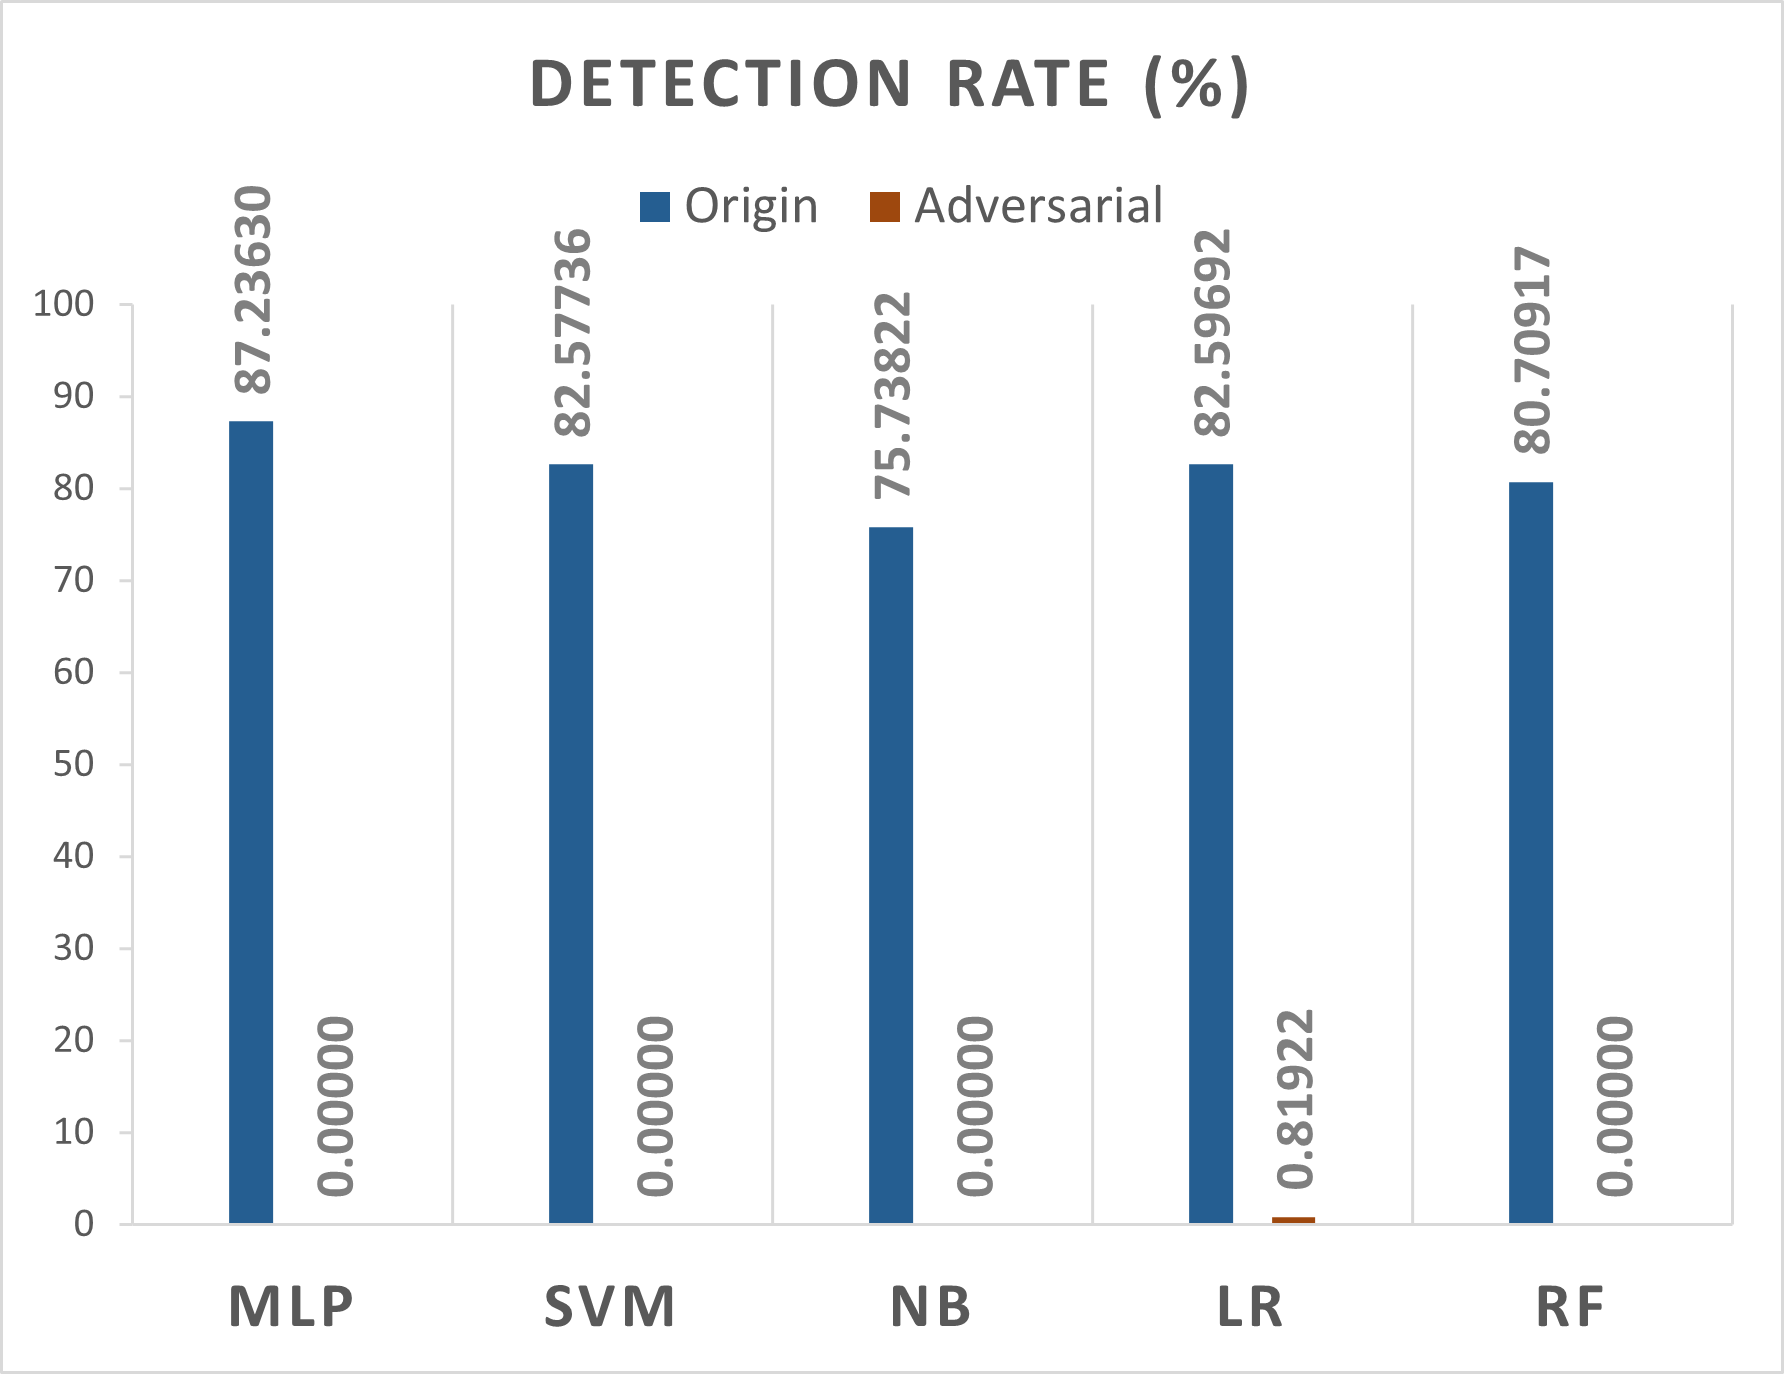
\includegraphics[width=.95\columnwidth]{Figures/UNSW-NB15}
    \caption{\label{fig:unsw-nb15-adversarial} \textit{UNSW-NB15} detection rate.}
\end{figure}

% ========================================================================== CIC-IDS2017
\begin{table}[t]
    \resizebox{\columnwidth}{!}{%
        \begin{tabular}{r|ll|ll|l}
            \cline{2-5}
            \multicolumn{1}{l|}{} & \multicolumn{2}{c|}{\textbf{Accuracy (\%)}} & \multicolumn{2}{c|}{\textbf{Detection Rate (\%)}} &  \\ \cline{2-6}
            \multicolumn{1}{l|}{} & \multicolumn{1}{c}{\textbf{Origin}} & \multicolumn{1}{c|}{\textbf{Adversarial}} & \multicolumn{1}{c}{\textbf{Origin}} & \multicolumn{1}{c|}{\textbf{Adversarial}} & \multicolumn{1}{c|}{\textbf{EIR}} \\ \hline
            \multicolumn{1}{|r|}{\textbf{MLP}} & 89.70249 & 43.17501 & 97.80681 & 0.00000 & \multicolumn{1}{l|}{1.00000} \\
            \multicolumn{1}{|r|}{\textbf{SVM}} & 93.95127 & 48.35813 & 95.48084 & 0.00000 & \multicolumn{1}{l|}{1.00000} \\
            \multicolumn{1}{|r|}{\textbf{NB}} & 97.83296 & 47.85404 & 95.74709 & 0.00000 & \multicolumn{1}{l|}{1.00000} \\
            \multicolumn{1}{|r|}{\textbf{LR}} & 92.30762 & 47.07897 & 93.84646 & 0.00000 & \multicolumn{1}{l|}{1.00000} \\
            \multicolumn{1}{|r|}{\textbf{RF}} & 97.92636 & 54.34136 & 91.54804 & 0.00000 & \multicolumn{1}{l|}{1.00000} \\ \hline
        \end{tabular}
    }
    \caption{Performance of the \textit{IDSs} classifiers with adversarial traffic on the \textit{CIC-IDS2017} dataset.
    \label{tab:adversarial-ids-classifiers-cic-ids-2017}}
\end{table}

\begin{figure}
    \centering
    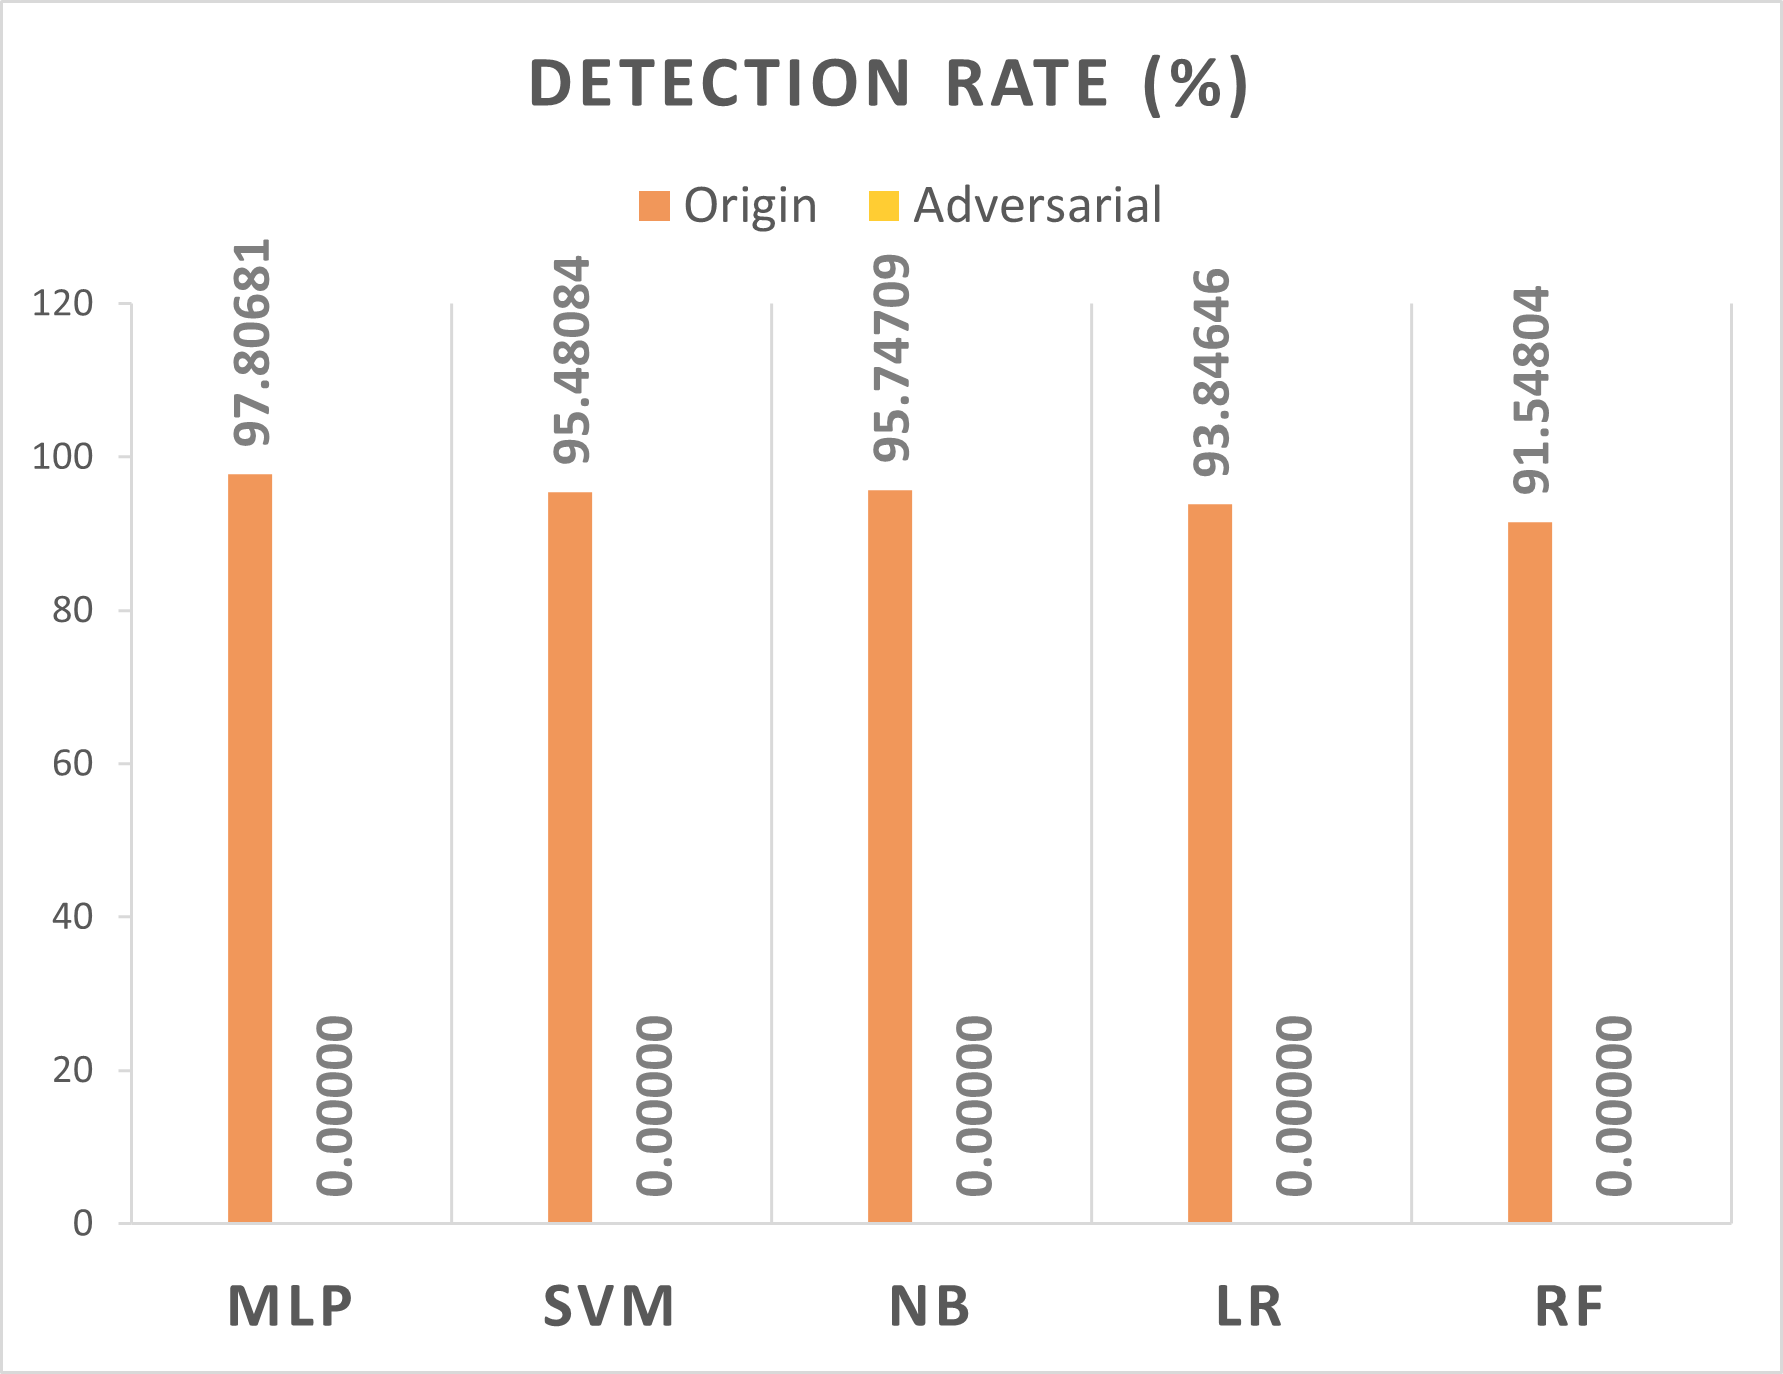
\includegraphics[width=.95\columnwidth]{Figures/CIC-IDS-2017}
    \caption{\label{fig:cic-ids2017-adversarial} \textit{CIC-IDS2017} detection rate.}
\end{figure}

% ========================================================================== CSE-CIC-IDS2018
\begin{table}[t]
    \resizebox{\columnwidth}{!}{%
        \begin{tabular}{r|ll|ll|l}
            \cline{2-5}
            \multicolumn{1}{l|}{} & \multicolumn{2}{c|}{\textbf{Accuracy (\%)}} & \multicolumn{2}{c|}{\textbf{Detection Rate (\%)}} &  \\ \cline{2-6}
            \multicolumn{1}{l|}{} & \multicolumn{1}{c}{\textbf{Origin}} & \multicolumn{1}{c|}{\textbf{Adversarial}} & \multicolumn{1}{c}{\textbf{Origin}} & \multicolumn{1}{c|}{\textbf{Adversarial}} & \multicolumn{1}{c|}{\textbf{EIR}} \\ \hline
            \multicolumn{1}{|r|}{\textbf{MLP}} & 89.03803 & 47.04617 & 94.76926 & 0.03464 & \multicolumn{1}{l|}{0.99963} \\
            \multicolumn{1}{|r|}{\textbf{SVM}} & 95.45637 & 45.35497 & 91.99673 & 0.00000 & \multicolumn{1}{l|}{1.00000} \\
            \multicolumn{1}{|r|}{\textbf{NB}} & 96.72028 & 48.55712 & 92.82482 & 0.00000 & \multicolumn{1}{l|}{1.00000} \\
            \multicolumn{1}{|r|}{\textbf{LR}} & 91.52872 & 44.39624 & 97.91123 & 0.47354 & \multicolumn{1}{l|}{0.99516} \\
            \multicolumn{1}{|r|}{\textbf{RF}} & 98.20424 & 56.16009 & 98.97865 & 0.00000 & \multicolumn{1}{l|}{1.00000} \\ \hline
        \end{tabular}
    }
    \caption{Performance of the \textit{IDSs} classifiers with adversarial traffic on the \textit{CSE-CIC-IDS2018} dataset.
    \label{tab:adversarial-ids-classifiers-cic-ids-2018}}
\end{table}

\begin{figure}
    \centering
    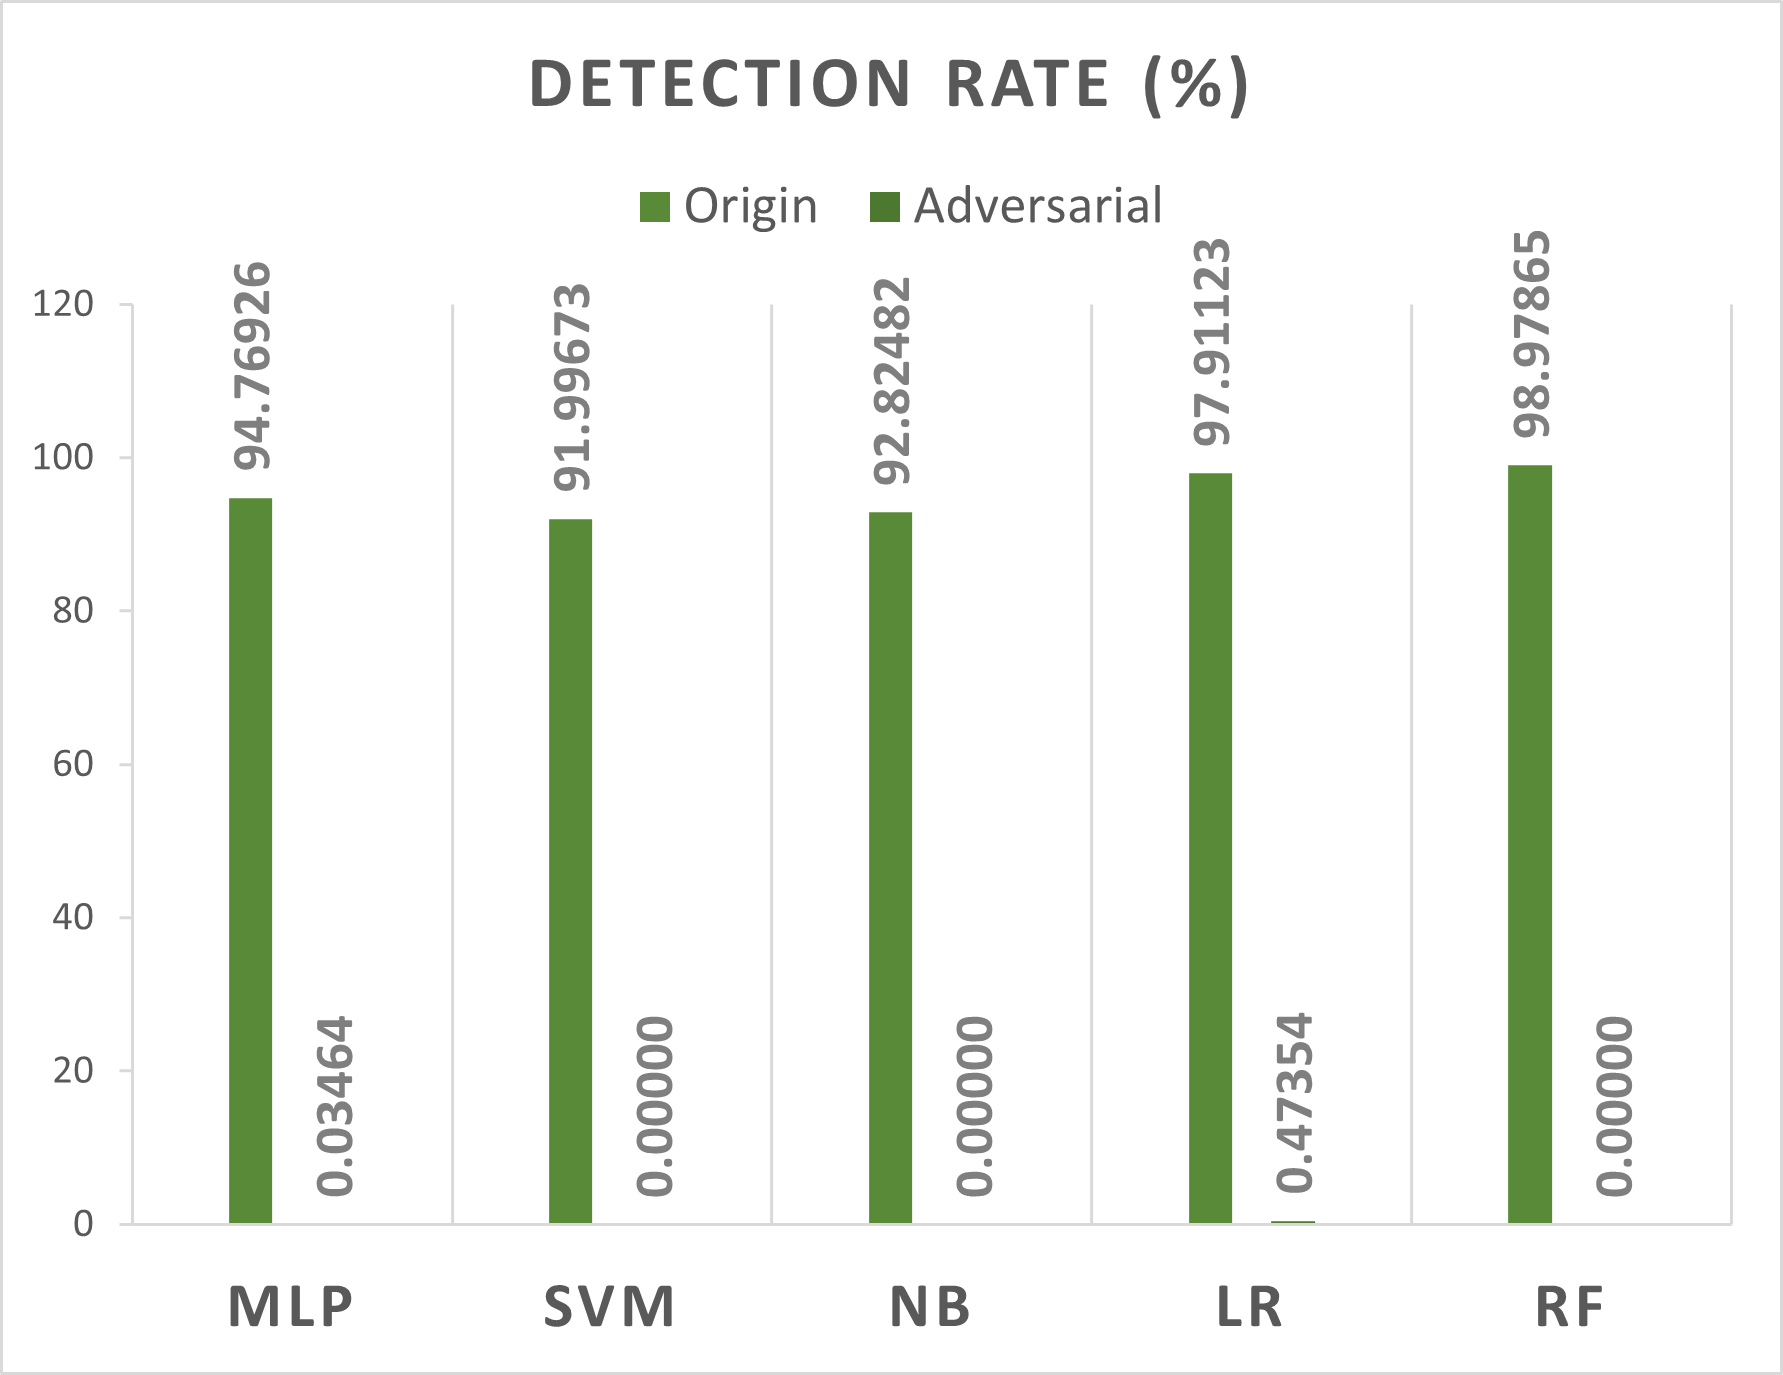
\includegraphics[width=.95\columnwidth]{Figures/CIC-IDS-2018}
    \caption{\label{fig:cic-ids2018-adversarial} \textit{CSE-CIC-IDS2018} detection rate.}
\end{figure}
% ========================================================================== CIC-DDoS2019
\begin{table}[t]
    \resizebox{\columnwidth}{!}{%
        \begin{tabular}{r|ll|ll|l}
            \cline{2-5}
            \multicolumn{1}{l|}{} & \multicolumn{2}{c|}{\textbf{Accuracy (\%)}} & \multicolumn{2}{c|}{\textbf{Detection Rate (\%)}} &  \\ \cline{2-6}
            \multicolumn{1}{l|}{} & \multicolumn{1}{c}{\textbf{Origin}} & \multicolumn{1}{c|}{\textbf{Adversarial}} & \multicolumn{1}{c}{\textbf{Origin}} & \multicolumn{1}{c|}{\textbf{Adversarial}} & \multicolumn{1}{c|}{\textbf{EIR}} \\ \hline
            \multicolumn{1}{|r|}{\textbf{MLP}} & 87.73115 & 48.70946 & 87.06869 & 0.00000 & \multicolumn{1}{l|}{1.00000} \\
            \multicolumn{1}{|r|}{\textbf{SVM}} & 85.45995 & 44.68655 & 84.43590 & 0.00000 & \multicolumn{1}{l|}{1.00000} \\
            \multicolumn{1}{|r|}{\textbf{NB}} & 86.16776 & 47.13445 & 85.14369 & 0.00000 & \multicolumn{1}{l|}{1.00000} \\
            \multicolumn{1}{|r|}{\textbf{LR}} & 83.96291 & 45.23399 & 85.20754 & 0.00000 & \multicolumn{1}{l|}{1.00000} \\
            \multicolumn{1}{|r|}{\textbf{RF}} & 91.42235 & 46.93493 & 84.20779 & 0.00000 & \multicolumn{1}{l|}{1.00000} \\ \hline
        \end{tabular}
    }
    \caption{Performance of the \textit{IDSs} classifiers with adversarial traffic on the \textit{CIC-DDoS2019} dataset.
    \label{tab:adversarial-ids-classifiers-cic-ids-2019}}
\end{table}

\begin{figure}
    \centering
    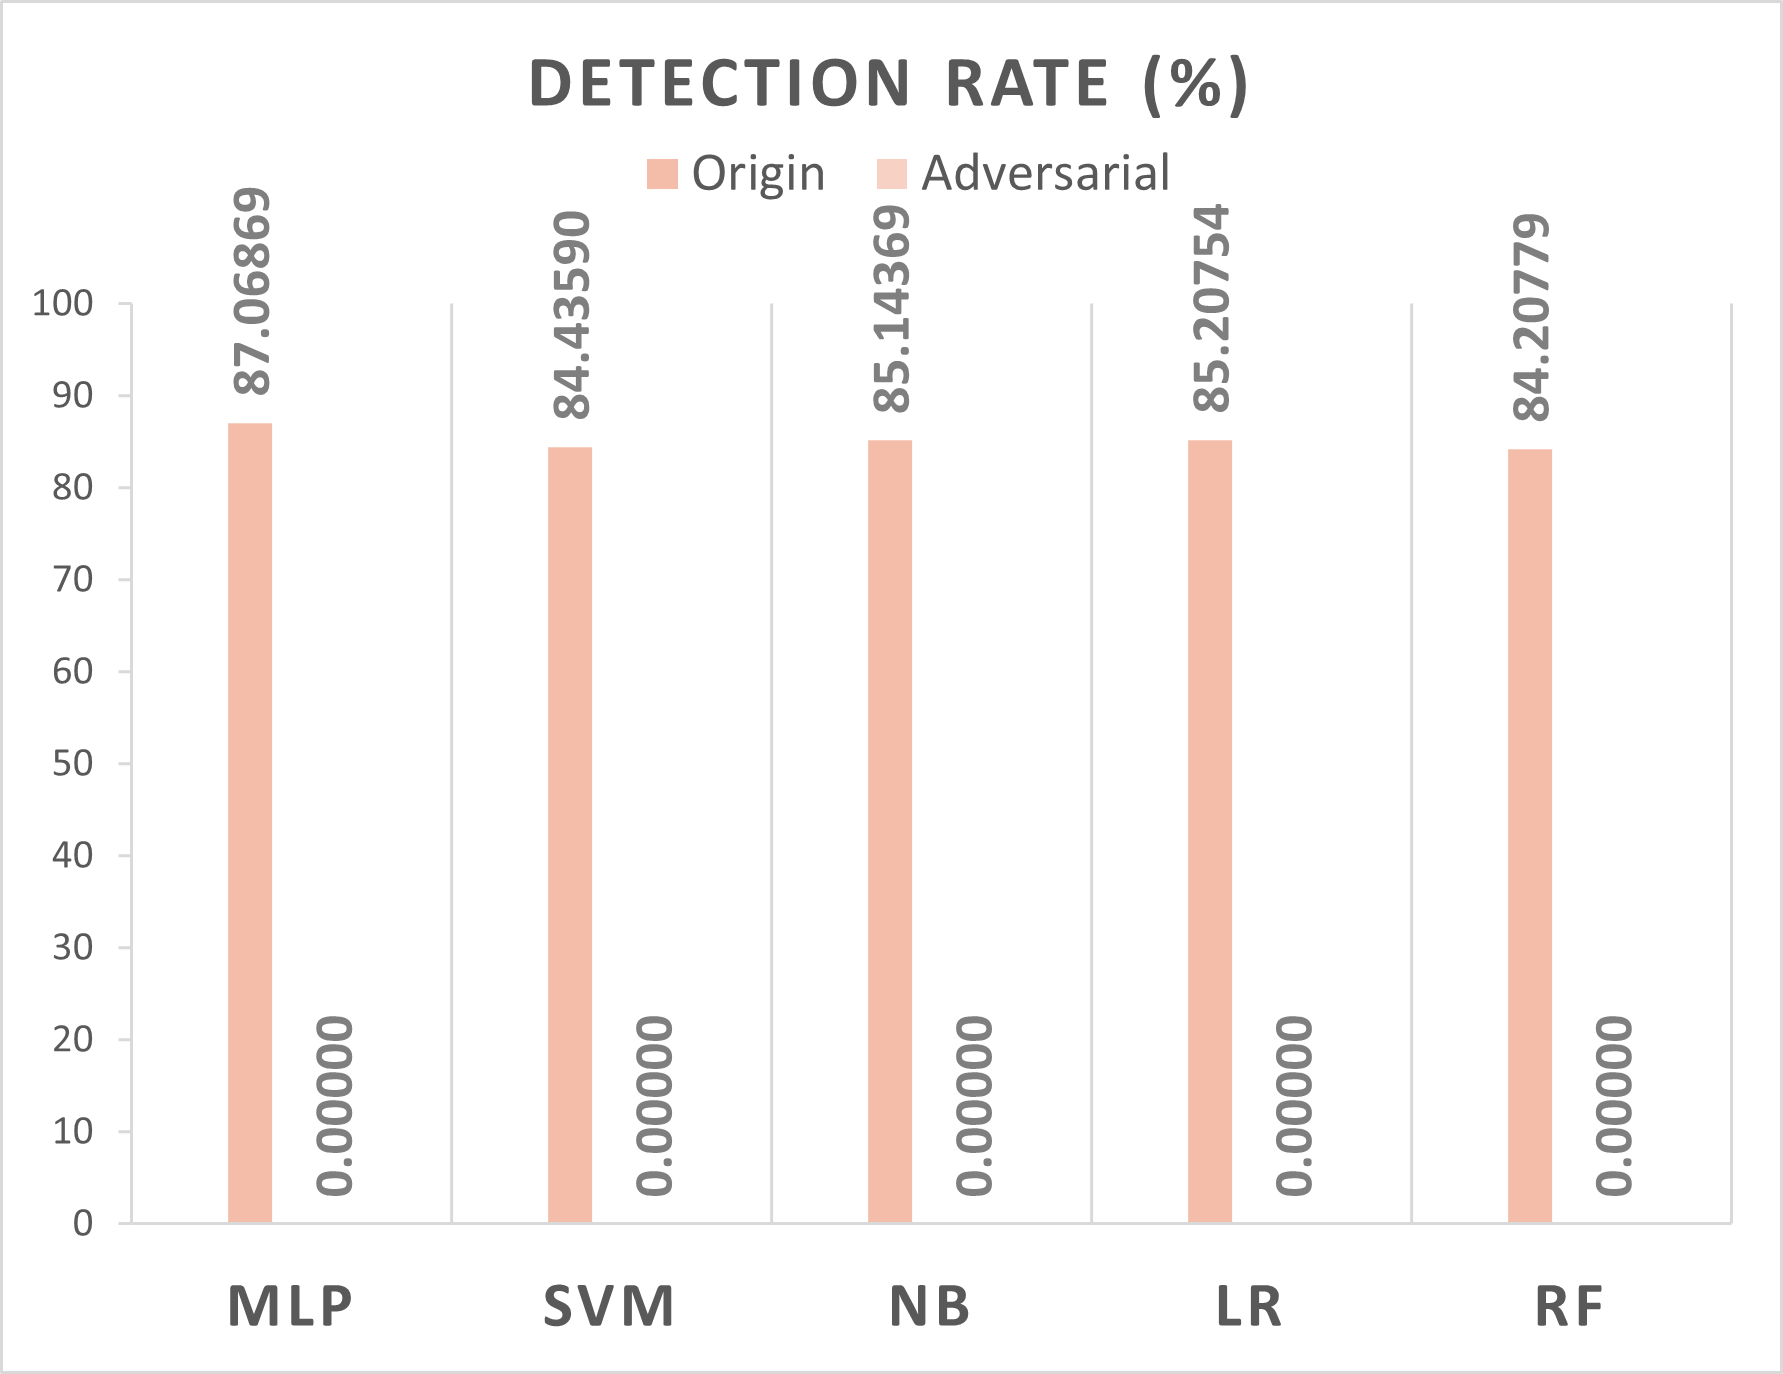
\includegraphics[width=.95\columnwidth]{Figures/CIC-IDS-2019}
    \caption{\label{fig:cic-ids2019-adversarial} \textit{CIC-DDoS2019} detection rate.}
\end{figure}

In this study, we begin our analysis with the \textit{UNSW-NB15} dataset.
The results of this analysis can be observed in Table~\ref{tab:adversarial-ids-classifiers-unsw-nb15} and in the
Figure~\ref{fig:unsw-nb15-adversarial}.
From the table, it is clear to see that the \textit{Detection Rate (DR)} and \textit{Evasion Increase Rate (EIR)}
metrics are quite high.
This indicates that almost all the adversarial traffic generated with our \textit{Harpe} framework is able to fool all
the \textit{IDS} models, and is able to evade detection as an attack.

In the \textit{CIC-IDS2017} (Table~\ref{tab:adversarial-ids-classifiers-cic-ids-2017} and
Figure~\ref{fig:cic-ids2017-adversarial}), \textit{CSE-CIC-IDS2018}
(Table~\ref{tab:adversarial-ids-classifiers-cic-ids-2018} and Figure~\ref{fig:cic-ids2018-adversarial})
and \textit{CIC-DDoS2019} (Table~\ref{tab:adversarial-ids-classifiers-cic-ids-2019} and
Figure~\ref{fig:cic-ids2019-adversarial})
datasets, as in the previous dataset, we can see how by generating adversarial network traffic with the \textit{Harpe}
framework we greatly reduce the \textit{Detection Rate} and obtain values very close to the maximum in the
\textit{Evasion Increase Rate}.
As a consequence, the \textit{accuracy} of the IDS classification algorithms is greatly reduced.

These results indicate that the \textit{Harpe} framework is able to successfully create adversarial attacks on network
traffic that are practically undetectable by the majority of traditional \textit{IDS} systems,
as well as other solutions such as \textit{IDSGAN}, \textit{attackGAN}, and \textit{DIGFuPAS}.
This is a significant achievement as it highlights the framework's ability to bypass the security measures put in place
by these systems.

\subsubsection{SDP IDS Environment}
In order to test our solution in an \textit{SDP-based} network environment, we needed to generate our dataset.
To do this, we developed a tool that simulates traffic in an \textit{SDP network} from two
\textit{SDP Initiating Hosts (IH)} to one \textit{SDP Accepting Host (AH)} using an \textit{Apache} web server.
In an \textit{SDP} network, a connection between an \textit{SDP IH} and an \textit{SDP AH} must be authorized by the
\textit{SDP Controller} prior to any communication taking place.
Because of this, we only stored authentication requests in our dataset, as they are the only type of requests that can
be targeted by attacks.

In general, once a connection is authorized, the \textit{SDP IH} is authorized to access the \textit{SDP AH} for as
long as the \textit{SDP controller} specifies or until the \textit{SDP IH} changes some of its characteristics, such as
IP address, geolocation, etc.
This results in very few authorization requests for the \textit{SDP IH}.
This results in very few authorization requests for a test environment such as the one in this project, where there are
only two \textit{SDP IHs}.
For this reason, we have configured the \textit{SDP Controller} so that the \textit{SDP IH} authorization only lasts
for one request.
This way the \textit{SDP IH} has to make an authorization request for each request it wants to make to the
\textit{SDP AH} web server.

Once we can generate normal or benign traffic, we need to generate attack traffic to train the \textit{grey/black-box}
\textit{IDS}.
To generate this attack traffic, we used the \textit{Slowloris}~\cite{damon2012hands} attack.
\textit{Slowloris} is a type of \textit{DoS} attack that is used to target web servers.
The attack works by consuming all of the available connections on a web server, making it unable to serve legitimate
requests.
This is accomplished by the attacker opening a large number of connections to the web server and keeping them open for
as long as possible.

The generated \textit{SDP}-based network traffic dataset is completely open and can be found in the
\textit{GitHub} repository.
The dataset is composed of two files in \textit{CSV} format, one with the benign traffic and the other with the traffic
generated when executing a \textit{Slowloris DoS} attack.
The dataset has 84 network flow features extracted from the \textit{pcap} files with full packet payloads using the
\textit{CICFlowmeter-V4.0} tool.
The subset with the benign data has 2193 authentication requests made from two \textit{SPD IHs}.
The subset with malicious data has 1203 requests made on one of the \textit{SPD IHs} without prior authentication.

Table~\ref{tab:adversarial-ids-classifiers-sdp} describes the results obtained after training the ML-based \textit{IDS}
for the \textit{SDP-based} network and their \textit{Detection Rates (DR)} for data generated with \textit{Harpe}.
In this scenario, we were only able to achieve detection rates close to 50\% during the training of the \textit{IDS}
classification models.
This may be due to the small amount of data available, as well as to the small variation between them (only two devices
make authentication requests, and one of these devices is the one that subsequently performs the attacks).
However, in real environments and with a larger number of devices, we assume that \textit{IDSs} can achieve much higher
\textit{DR} scores.

\begin{table}[t]
    \resizebox{\columnwidth}{!}{%
        \begin{tabular}{r|ll|ll|l}
            \cline{2-5}
            \multicolumn{1}{l|}{} & \multicolumn{2}{c|}{\textbf{Accuracy (\%)}} & \multicolumn{2}{c|}{\textbf{Detection Rate (\%)}} &  \\ \cline{2-6}
            \multicolumn{1}{l|}{} & \multicolumn{1}{c}{\textbf{Origin}} & \multicolumn{1}{c|}{\textbf{Adversarial}} & \multicolumn{1}{c}{\textbf{Origin}} & \multicolumn{1}{c|}{\textbf{Adversarial}} & \multicolumn{1}{c|}{\textbf{EIR}} \\ \hline
            \multicolumn{1}{|r|}{\textbf{MLP}} & 76.35870 & 49.68038 & 52.71739 & 20.03842 & \multicolumn{1}{l|}{0.61989} \\
            \multicolumn{1}{|r|}{\textbf{SVM}} & 72.75557 & 64.00435 & 37.43255 & 17.10665 & \multicolumn{1}{l|}{0.54300} \\
            \multicolumn{1}{|r|}{\textbf{NB}} & 56.04148 & 55.26820 & 41.92895 & 1.25832 & \multicolumn{1}{l|}{0.96999} \\
            \multicolumn{1}{|r|}{\textbf{LR}} & 68.30679 & 45.23399 & 40.49852 & 8.04726 & \multicolumn{1}{l|}{0.80130} \\
            \multicolumn{1}{|r|}{\textbf{RF}} & 75.28038 & 57.34791 & 55.13747 & 29.51201 & \multicolumn{1}{l|}{0.46476} \\ \hline
        \end{tabular}
    }
    \caption{Performance of the \textit{IDSs} classifiers with adversarial traffic on the generated \textit{SDP}-based network dataset.
    \label{tab:adversarial-ids-classifiers-sdp}}
\end{table}

\begin{figure}
    \centering
    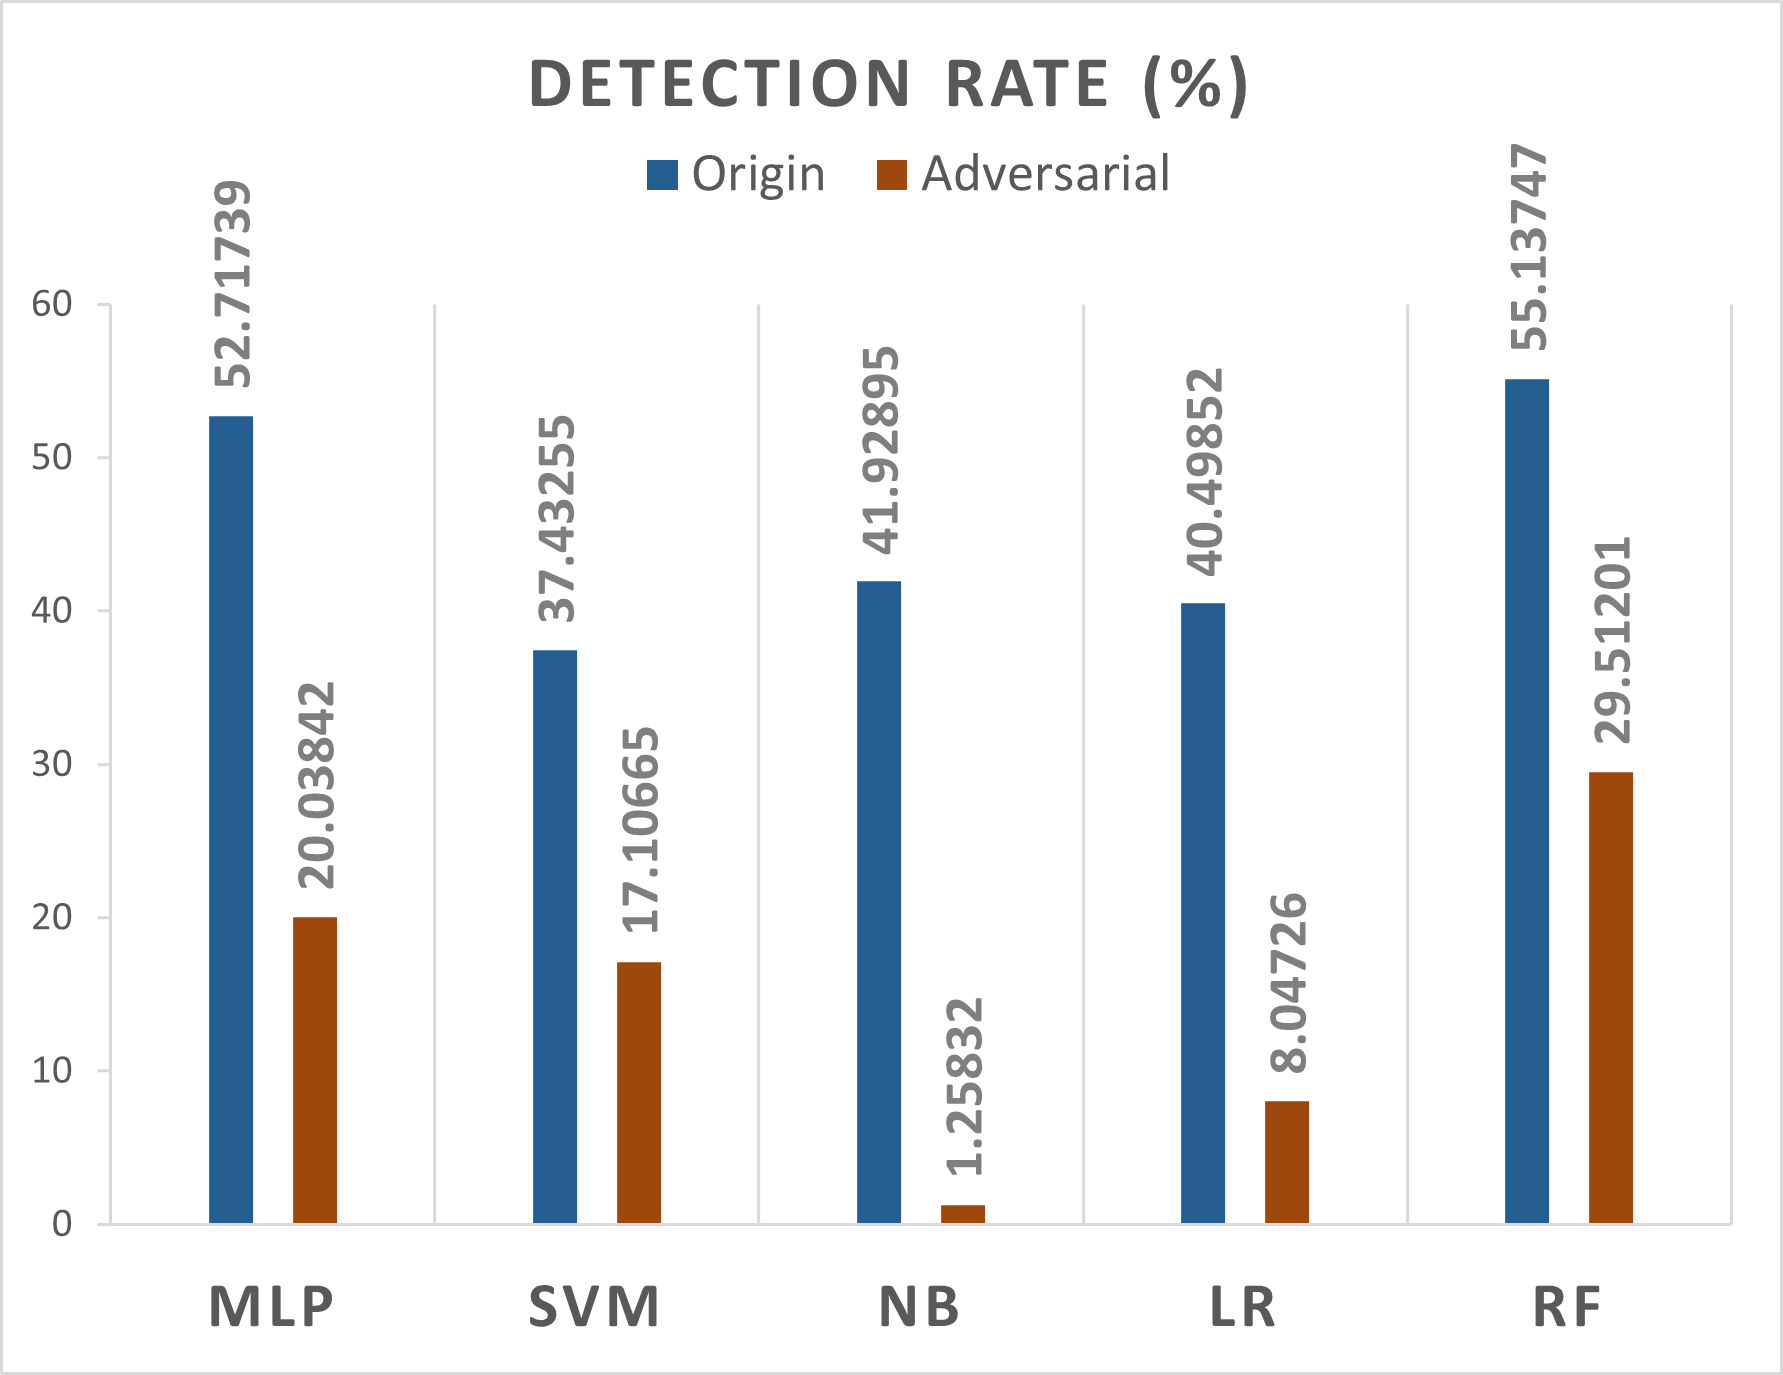
\includegraphics[width=.95\columnwidth]{Figures/SDP-Dataset}
    \caption{\label{fig:dataset-sdp} \textit{SDP}-based network generated dataset detection rate.}
\end{figure}

In this environment, \textit{Harpe} is able to significantly reduce the ability of an \textit{IDS} to distinguish
whether a request is a \textit{DoS} attack or a real authentication request, and performs better against classifiers
using \textit{NB} and \textit{LR}.
